\documentclass{beamer}
\usepackage{tikz,amsmath,hyperref,graphicx,stackrel,animate}
\usetikzlibrary{positioning,shadows,arrows,shapes,calc}
\newcommand{\argmax}{\operatornamewithlimits{argmax}}
\newcommand{\argmin}{\operatornamewithlimits{argmin}}
\mode<presentation>{\usetheme{Frankfurt}}
\AtBeginSection[]
{
  \begin{frame}<beamer>
    \frametitle{Outline}
    \tableofcontents[currentsection,currentsubsection]
  \end{frame}
}
\title{Lecture 7: Neural Nets}
\author{Mark Hasegawa-Johnson}
\date{ECE 417: Multimedia Signal Processing, Fall 2020}  
\begin{document}

% Title
\begin{frame}
  \maketitle
\end{frame}

% Title
\begin{frame}
  \tableofcontents
\end{frame}


%%%%%%%%%%%%%%%%%%%%%%%%%%%%%%%%%%%%%%%%%%%%
\section{Intro}
\setcounter{subsection}{1}
\begin{frame}
  \frametitle{What is a Neural Network?}
  \begin{itemize}
  \item Computation in biological neural networks is performed by
    trillions of simple cells (neurons), each of which performs one
    very simple computation.
  \item Biological neural networks learn by strengthening  the connections
    between some pairs of neurons, and weakening other connections.
  \end{itemize}
\end{frame}

\begin{frame}
  \frametitle{What is an Artificial Neural Network?}
  \begin{itemize}
  \item Computation in an artificial neural network is performed by
    thousands of simple cells (nodes), each of which performs one
    very simple computation.
  \item Artificial neural networks learn by strengthening  the connections
    between some pairs of nodes, and weakening other connections.
  \end{itemize}
\end{frame}

\begin{frame}
  \frametitle{Two-Layer Feedforward Neural Network}
  \begin{small}\begin{center}
  \tikzstyle{pre}=[<-,shorten <=1pt,>=stealth',semithick,draw=blue]
  \tikzstyle{post}=[->,shorten >=1pt,>=stealth',semithick,draw=blue]
  \begin{tikzpicture}[
      open/.style={circle,thick, draw=blue, text=black, align=left, text width=0.5cm}
    ]
    \node (x0) at (0,0.25) {$1$};
    \node[open] (x1) at (1,0) {$x_1$};
    \node[open] (x2) at (2,0) {$x_2$};
    \node (x3) at (2.75,0) {\ldots};
    \node[open] (xm0) at (3.5,0) {$x_{m_0}$};
    \node (input) at (6,0) {$\mathbf{a}_0=\mathbf{x}$ is the input vector};
    \node[open] (z11) at (1,1.3) {$z_{1,1}$} edge[pre](x0) edge[pre](x1) edge[pre](x2) edge[pre](xm0);
    \node[open] (z12) at (2,1.3) {$z_{1,2}$} edge[pre](x0) edge[pre](x1) edge[pre](x2) edge[pre](xm0);
    \node (z13) at (2.75,1.3) {\ldots};
    \node[open] (z1m1) at (3.5,1.3) {$z_{1,m_1}$} edge[pre](x0) edge[pre](x1) edge[pre](x2) edge[pre](xm0);
    \node (z1eq) at (6,1.3) {$\mathbf{z}_1=\mathbf{W}_1\mathbf{x}+\mathbf{b}_1$};
    \node (a10) at (0,2.7) {$1$};
    \node[open] (a11) at (1,2.45) {$a_{1,1}$} edge[pre](z11);
    \node[open] (a12) at (2,2.45) {$a_{1,2}$} edge[pre](z12);
    \node (a13) at (2.75,2.45) {\ldots};
    \node[open] (a1m1) at (3.5,2.45) {$a_{1,m_1}$} edge[pre](z1m1);
    \node (a1eq) at (6,2.45) {$\mathbf{a}_1=\mathbf{f}_1(\mathbf{z}_1)$};
    \node[open] (z21) at (1,3.75) {$z_{2,1}$} edge[pre](a10) edge[pre](a11) edge[pre](a12) edge[pre](a1m1);
    \node[open] (z22) at (2,3.75) {$z_{2,2}$} edge[pre](a10) edge[pre](a11) edge[pre](a12) edge[pre](a1m1);
    \node (z23) at (2.75,3.75) {\ldots};
    \node[open] (z2m2) at (3.5,3.75){$z_{2,m_2}$}edge[pre](a10) edge[pre](a11) edge[pre](a12) edge[pre](a1m1);
    \node (z2eq) at (6,3.75) {$\mathbf{z}_2=\mathbf{W}_2\mathbf{a}_1+\mathbf{b}_2$};
    \node[open] (a21) at (1,4.9) {$g_{1}$} edge[pre](z21);
    \node[open] (a22) at (2,4.9) {$g_{2}$} edge[pre](z22);
    \node (a23) at (2.75,4.9) {\ldots};
    \node[open] (a2m2) at (3.5,4.9) {$g_{m_2}$} edge[pre](z2m2);
    \node (z2eq) at (6,4.9) {$\mathbf{g}(\mathbf{x})=\mathbf{a}_2=\mathbf{f}_2(\mathbf{z}_2)$};
    \node (output) at (2.2,5.65) {${\mathcal{L}}=E\left[-\ln\Pr(\mathbf{y}|\mathbf{g}(\mathbf{x}))\right]$};
  \end{tikzpicture}
\end{center}
\end{small}
\end{frame}

\begin{frame}
  \frametitle{Neural Network = Universal Approximator}
  Assume\ldots
  \begin{itemize}
  \item Linear Output Nodes: $\hat{y}_k=e_k^{(2)}$
  \item Smoothly Nonlinear Hidden Nodes: $\frac{d\sigma}{de}$ finite
  \item Smooth Target Function: $\hat{y}=h(\vec{x},W,b)$ approximates
    $\vec{y}=h^*(\vec{x})\in{\mathcal H}$, where ${\mathcal H}$ is
    some class of sufficiently smooth functions of $\vec{x}$
    (functions whose Fourier transform has a first moment less than
    some finite number $C$)
    \item There are $N$ hidden nodes, $\hat{y}_k$, $1\le k\le N$
    \item The input vectors are distributed with some probability
      density function, $p(\vec{x})$, over which we can compute
      expected values.
  \end{itemize}
  Then (Barron, 1993) showed that\ldots
  \[
  \max_{h^*(\vec{x})\in{\mathcal H}}
    \min_{W,b} E\left[h(\vec{x},W,b)-h^*(\vec{x})\vert^2\right]
    \le {\mathcal O}\left\{\frac{1}{N}\right\}
    \]
\end{frame}

%%%%%%%%%%%%%%%%%%%%%%%%%%%%%%%%%%%%%%%%%%%%%%%%%%%%%%%%%%%%%%%
\section[Example \#1]{Example \#1: Neural Net as Universal Approximator}
\setcounter{subsection}{1}

\begin{frame}
  \frametitle{Target: Can we get the neural net to compute this
    function?}  Suppose our goal is to find some weights and biases,
  $W^{(1)}$, $\vec{b}^{(1)}$, $W^{(2)}$, and $\vec{b}^{(2)}$ so that
  $\hat{y}(\vec{x})$ is the nonlinear function shown here:
  \centerline{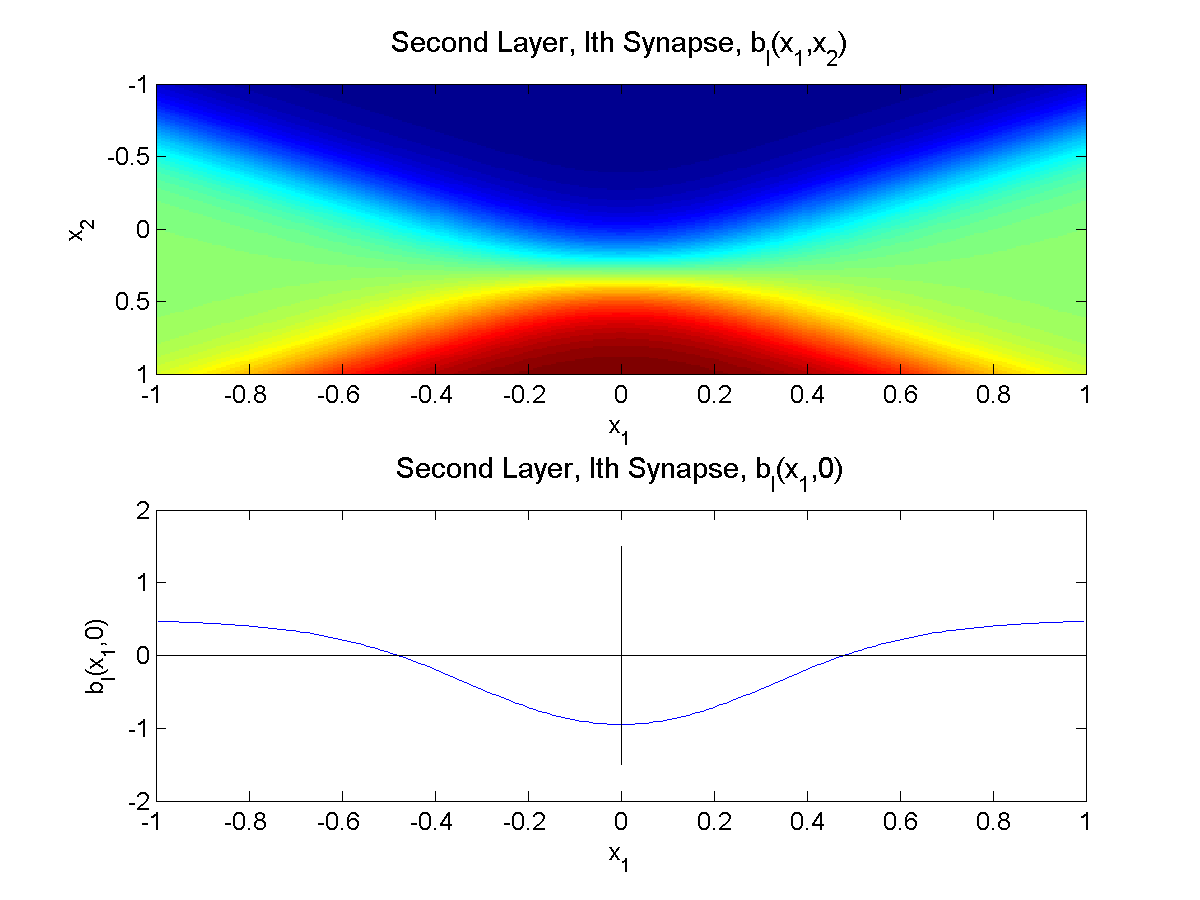
\includegraphics[width=3in]{figs/nn_synapse2.png}}
\end{frame}

\begin{frame}
  \frametitle{Excitation, First Layer:
    $e_k^{(1)}=b_{k}^{(1)}+\sum_{j=1}^2 w_{kj}^{(1)}x_j$} The first
  layer of the neural net just computes a linear function of
  $\vec{x}$. Here's an example:
  \centerline{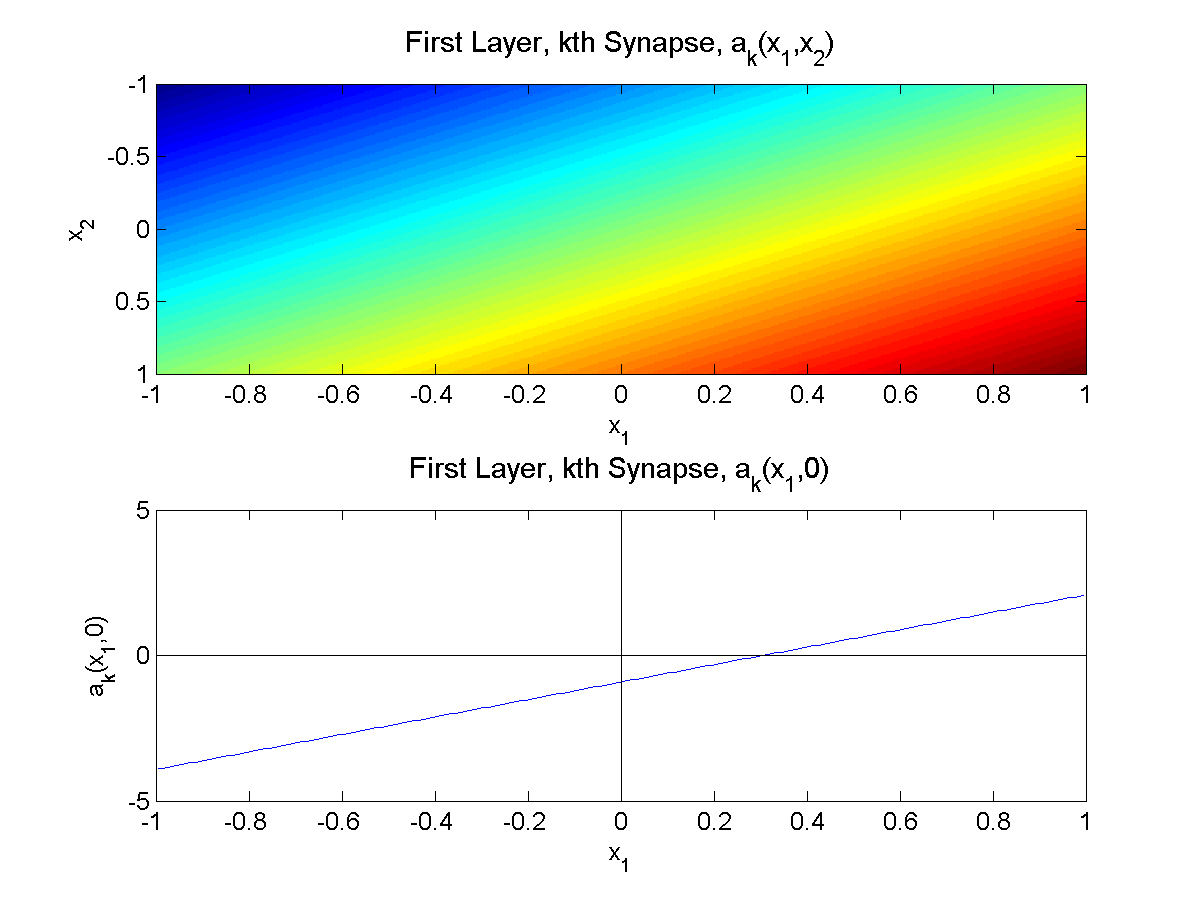
\includegraphics[width=3in]{figs/nn_synapse1.png}}
\end{frame}

\begin{frame}
  \frametitle{Activation, First Layer: $h_k=\tanh(e_k^{(1)})$} The
  activation nonlinearity then ``squashes'' the linear function:
  \centerline{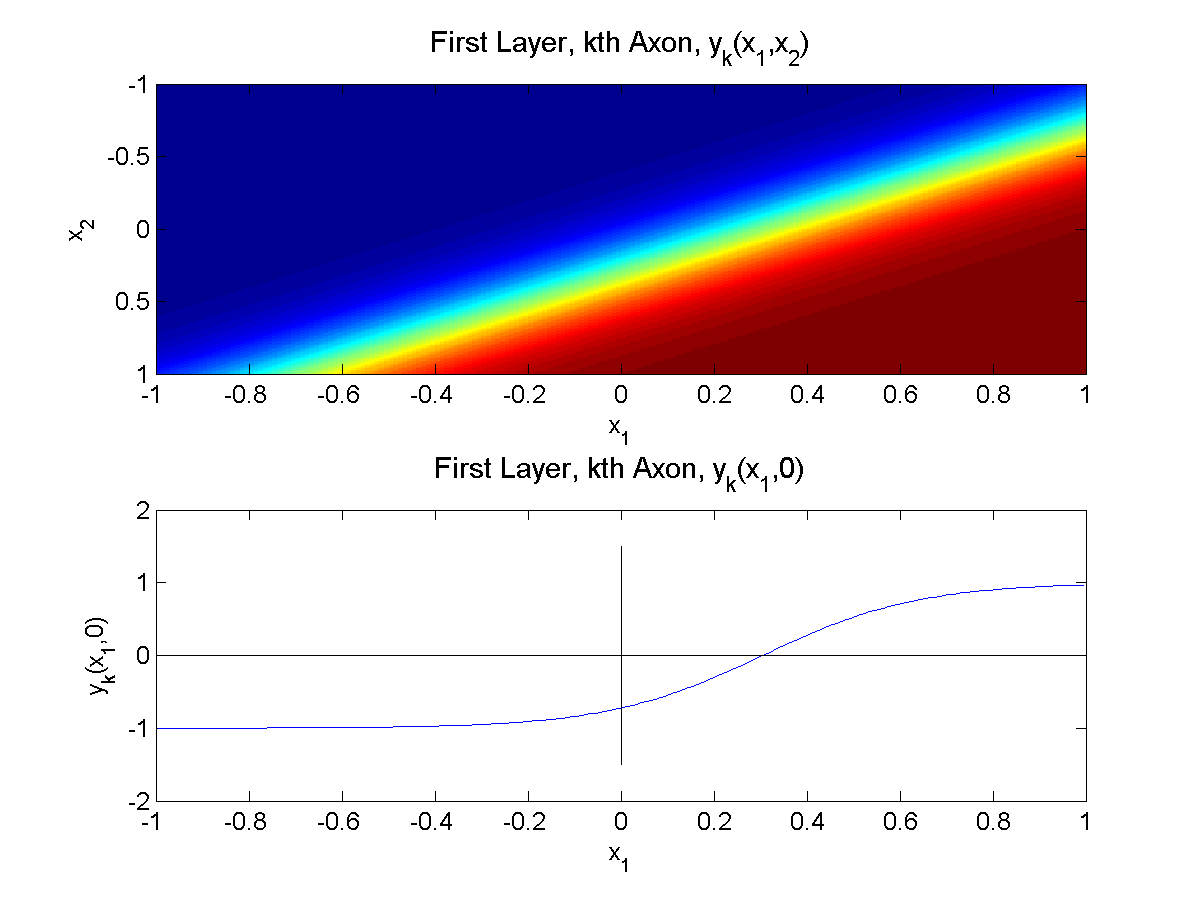
\includegraphics[width=3in]{figs/nn_axon1.png}}
\end{frame}

\begin{frame}
  \frametitle{Second Layer:
    $\hat{y}_k=b_{k}^{(2)}+\sum_{j=1}^2w_{kj}^{(2)}h_k$} The second
  layer then computes a linear combination of the first-layer
  activations, which is sufficient to match our desired function:
  \centerline{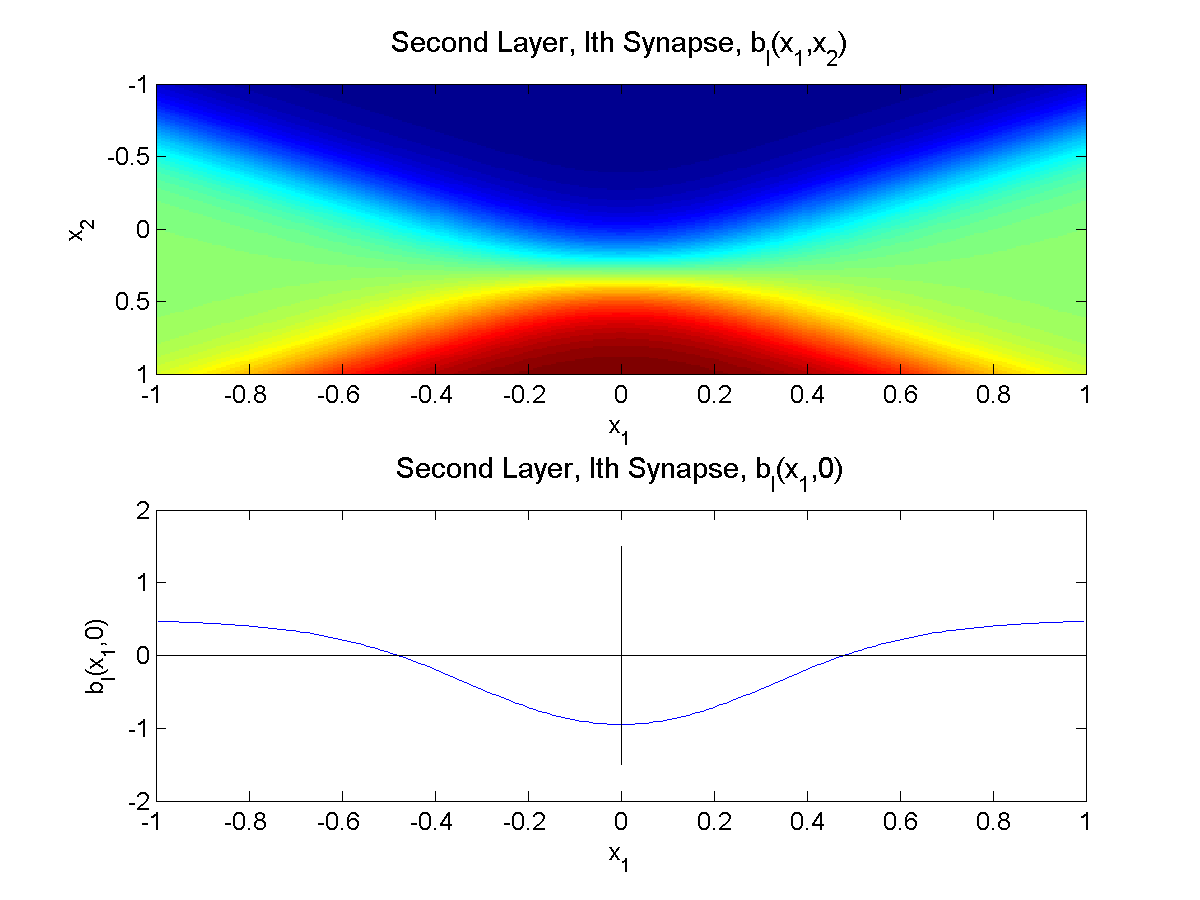
\includegraphics[width=3in]{figs/nn_synapse2.png}}
\end{frame}
%

%%%%%%%%%%%%%%%%%%%%%%%%%%%%%%%%%%%%%%%%%%%%%%%%%%%%%%%%%%%%%%%
\section[Example \#2]{Example \#2: Semicircle $\rightarrow$ Parabola}
\setcounter{subsection}{1}

\begin{frame}
  \frametitle{Example \#2: Semicircle $\rightarrow$ Parabola}

  Can we design a neural net that converts a semicircle
  ($x_0^2+x_1^2=1$) to a parabola ($y_1=y_0^2$)?
  \centerline{\includegraphics[height=2in]{exp/nn_target_figure.png}}
\end{frame}

\begin{frame}
  \frametitle{Two-Layer Feedforward Neural Network}
  \begin{small}\begin{center}
  \tikzstyle{pre}=[<-,shorten <=1pt,>=stealth',semithick,draw=blue]
  \tikzstyle{post}=[->,shorten >=1pt,>=stealth',semithick,draw=blue]
  \begin{tikzpicture}[
      open/.style={circle,thick, draw=blue, text=black, align=left, text width=0.5cm}
    ]
    \node (x0) at (0,0.25) {$1$};
    \node[open] (x1) at (1,0) {$x_1$};
    \node[open] (x2) at (2,0) {$x_2$};
    \node (x3) at (2.75,0) {\ldots};
    \node[open] (xm0) at (3.5,0) {$x_{m_0}$};
    \node (input) at (6,0) {$\mathbf{a}_0=\mathbf{x}$ is the input vector};
    \node[open] (z11) at (1,1.3) {$z_{1,1}$} edge[pre](x0) edge[pre](x1) edge[pre](x2) edge[pre](xm0);
    \node[open] (z12) at (2,1.3) {$z_{1,2}$} edge[pre](x0) edge[pre](x1) edge[pre](x2) edge[pre](xm0);
    \node (z13) at (2.75,1.3) {\ldots};
    \node[open] (z1m1) at (3.5,1.3) {$z_{1,m_1}$} edge[pre](x0) edge[pre](x1) edge[pre](x2) edge[pre](xm0);
    \node (z1eq) at (6,1.3) {$\mathbf{z}_1=\mathbf{W}_1\mathbf{x}+\mathbf{b}_1$};
    \node (a10) at (0,2.7) {$1$};
    \node[open] (a11) at (1,2.45) {$a_{1,1}$} edge[pre](z11);
    \node[open] (a12) at (2,2.45) {$a_{1,2}$} edge[pre](z12);
    \node (a13) at (2.75,2.45) {\ldots};
    \node[open] (a1m1) at (3.5,2.45) {$a_{1,m_1}$} edge[pre](z1m1);
    \node (a1eq) at (6,2.45) {$\mathbf{a}_1=\mathbf{f}_1(\mathbf{z}_1)$};
    \node[open] (z21) at (1,3.75) {$z_{2,1}$} edge[pre](a10) edge[pre](a11) edge[pre](a12) edge[pre](a1m1);
    \node[open] (z22) at (2,3.75) {$z_{2,2}$} edge[pre](a10) edge[pre](a11) edge[pre](a12) edge[pre](a1m1);
    \node (z23) at (2.75,3.75) {\ldots};
    \node[open] (z2m2) at (3.5,3.75){$z_{2,m_2}$}edge[pre](a10) edge[pre](a11) edge[pre](a12) edge[pre](a1m1);
    \node (z2eq) at (6,3.75) {$\mathbf{z}_2=\mathbf{W}_2\mathbf{a}_1+\mathbf{b}_2$};
    \node[open] (a21) at (1,4.9) {$g_{1}$} edge[pre](z21);
    \node[open] (a22) at (2,4.9) {$g_{2}$} edge[pre](z22);
    \node (a23) at (2.75,4.9) {\ldots};
    \node[open] (a2m2) at (3.5,4.9) {$g_{m_2}$} edge[pre](z2m2);
    \node (z2eq) at (6,4.9) {$\mathbf{g}(\mathbf{x})=\mathbf{a}_2=\mathbf{f}_2(\mathbf{z}_2)$};
    \node (output) at (2.2,5.65) {${\mathcal{L}}=E\left[-\ln\Pr(\mathbf{y}|\mathbf{g}(\mathbf{x}))\right]$};
  \end{tikzpicture}
\end{center}
\end{small}
\end{frame}

\begin{frame}
  \frametitle{Example \#2: Semicircle $\rightarrow$ Parabola}

  Let's define some vector notation:
  \begin{itemize}
  \item {\bf Second Layer:} Define
    $\vec{w}_j^{(2)}=\left[\begin{array}{c}w_{0j}^{(2)}\\w_{1j}^{(2)}\end{array}\right]$,
    the $j^{\textrm{th}}$ column of the $W^{(2)}$ matrix, so that
    \[
    \hat{y} = \vec{b} + \sum_j \vec{w}_{j}^{(2)} h_j~~~\mbox{means}~~~
    \hat{y}_k = b_k + \sum_j w_{kj}^{(2)} h_j\forall k.
    \]
  \item {\bf First Layer Activation Function:}
    \[
    h_k = \sigma\left(e_k^{(1)}\right)
    \]
  \item {\bf First Layer Excitation:} Define
    $\bar{w}_k^{(1)}=[w_{k0}^{(1)},w_{k1}^{(1)}]$, the
    $k^{\textrm{th}}$ row of the $W^{(1)}$ matrix, so that
    \[
    e_k^{(1)} = \bar{w}_{k}^{(1)} \vec{x}~~~\mbox{means}~~~
    e_k^{(1)} = \sum_j w_{kj}^{(1)} x_j\forall k.
    \]
  \end{itemize}
\end{frame}

\begin{frame}
  \frametitle{Second Layer = Piece-Wise Approximation}

  The second layer of the network approximates $\hat{y}$ using a bias term $\vec{b}$,
  plus correction vectors $\vec{w}_j^{(2)}$, each scaled by its activation $h_j$:
  \[
  \hat{y} = \vec{b}^{(2)} + \sum_j \vec{w}_{j}^{(2)} h_j
  \]
  The activation, $h_j$, is a number between 0 and 1.  For example, we could
  use the logistic sigmoid function:
  \[
  h_k = \sigma\left(e_k^{(1)}\right)=\frac{1}{1+\exp(-e_k^{(1)})}\in\left(0,1\right)
  \]
  The logistic sigmoid is a differentiable approximation to a unit step function.
\end{frame}

\begin{frame}
  \begin{columns}[t]
    \column{2.25in}
    \begin{block}{Step and Logistic nonlinearities}
      \centerline{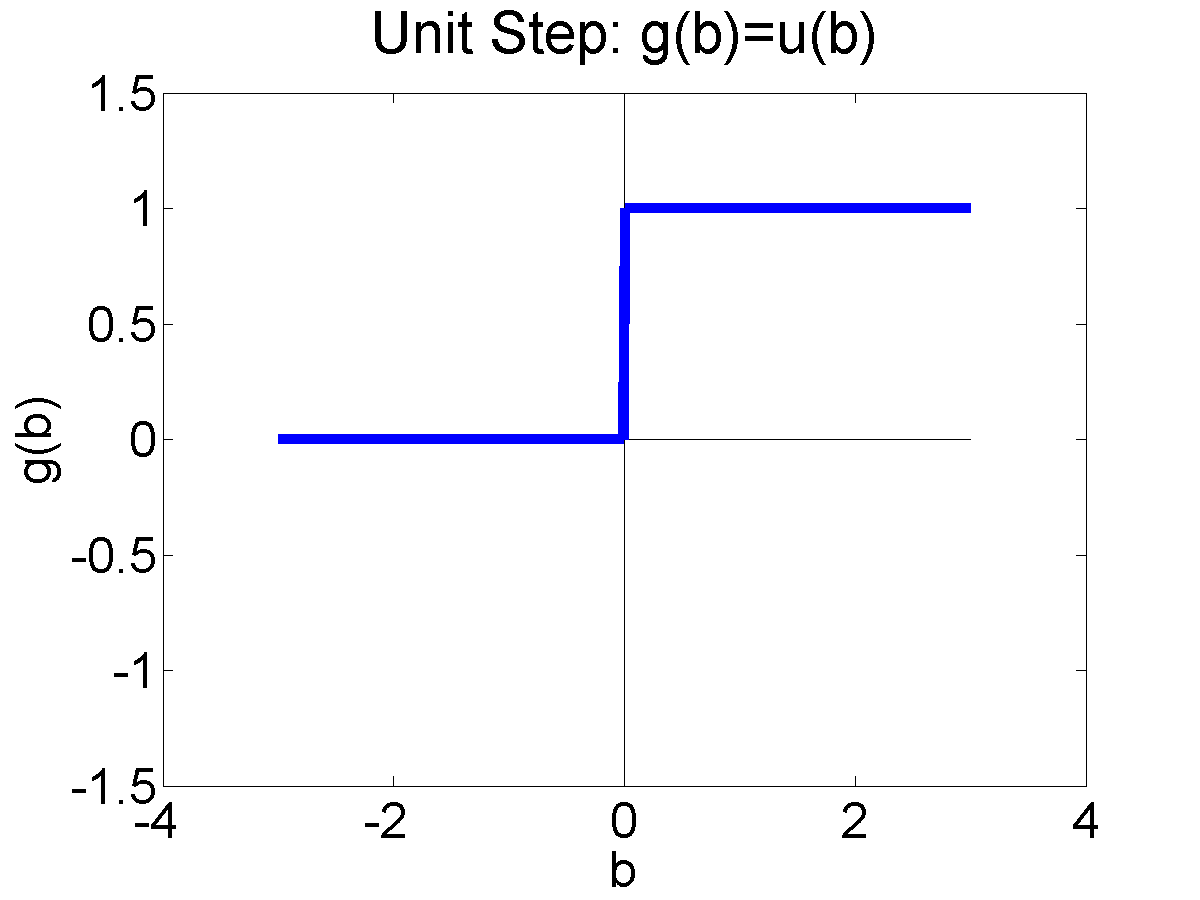
\includegraphics[width=1.75in]{figs/nn_unitstep.png}}
      \centerline{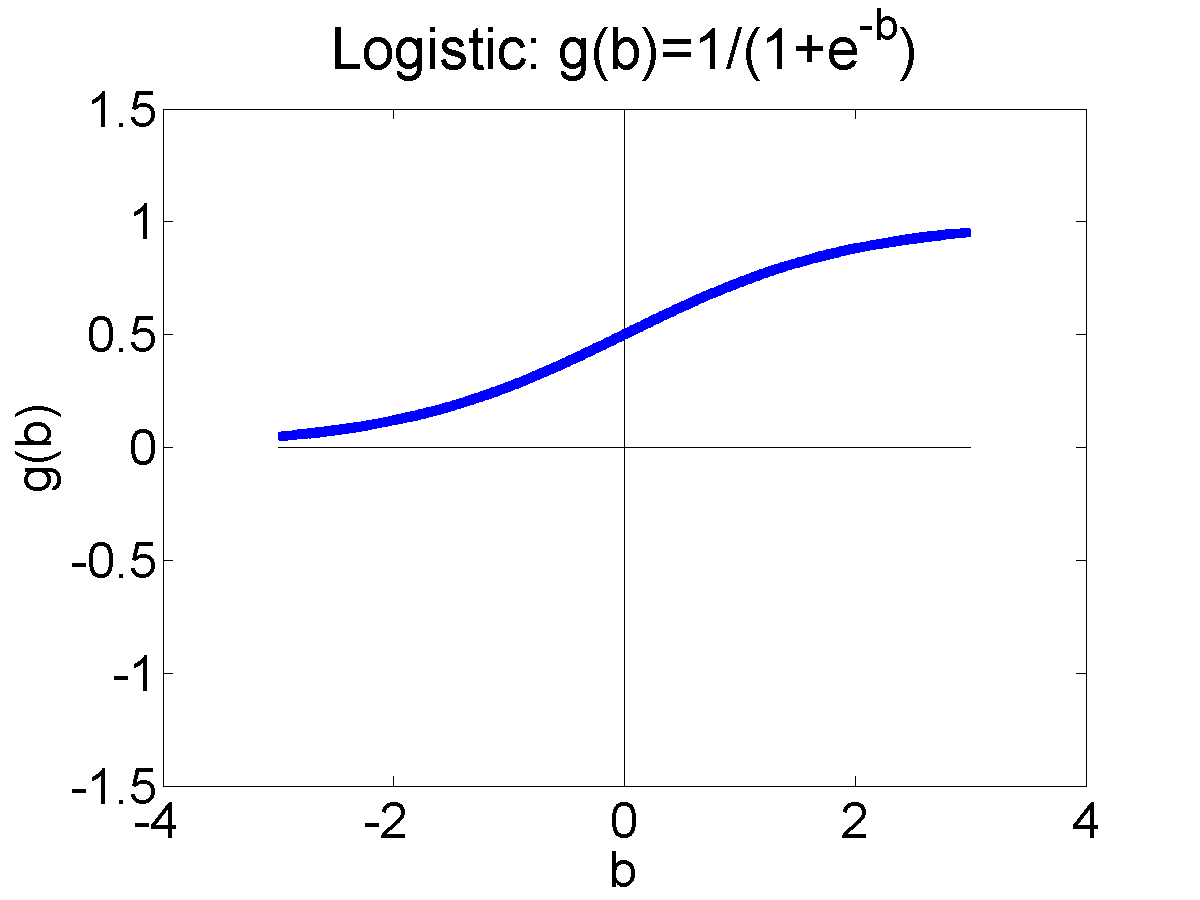
\includegraphics[width=1.75in]{figs/nn_logistic.png}}
    \end{block}
    \column{2.25in}
    \begin{block}{Signum and Tanh nonlinearities}
      \centerline{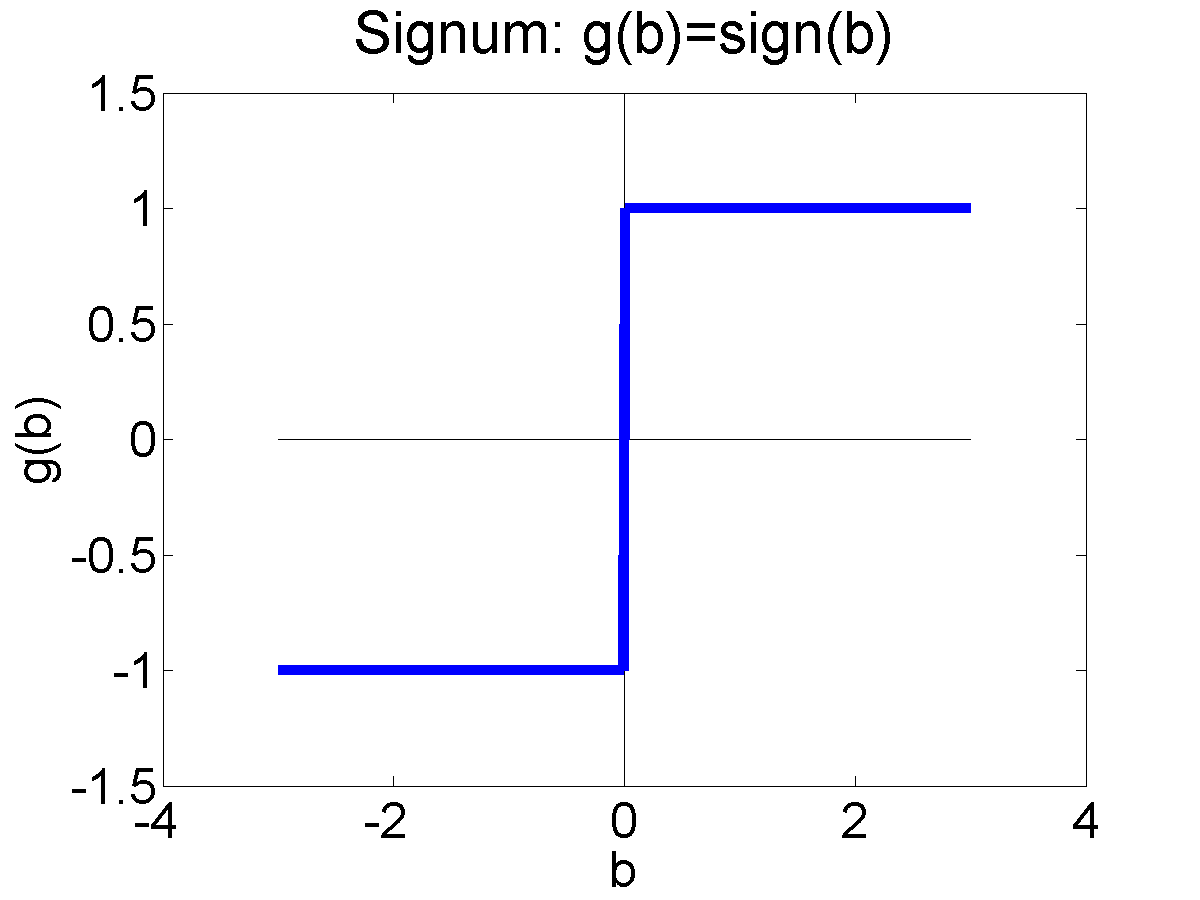
\includegraphics[width=1.75in]{figs/nn_signum.png}}
      \centerline{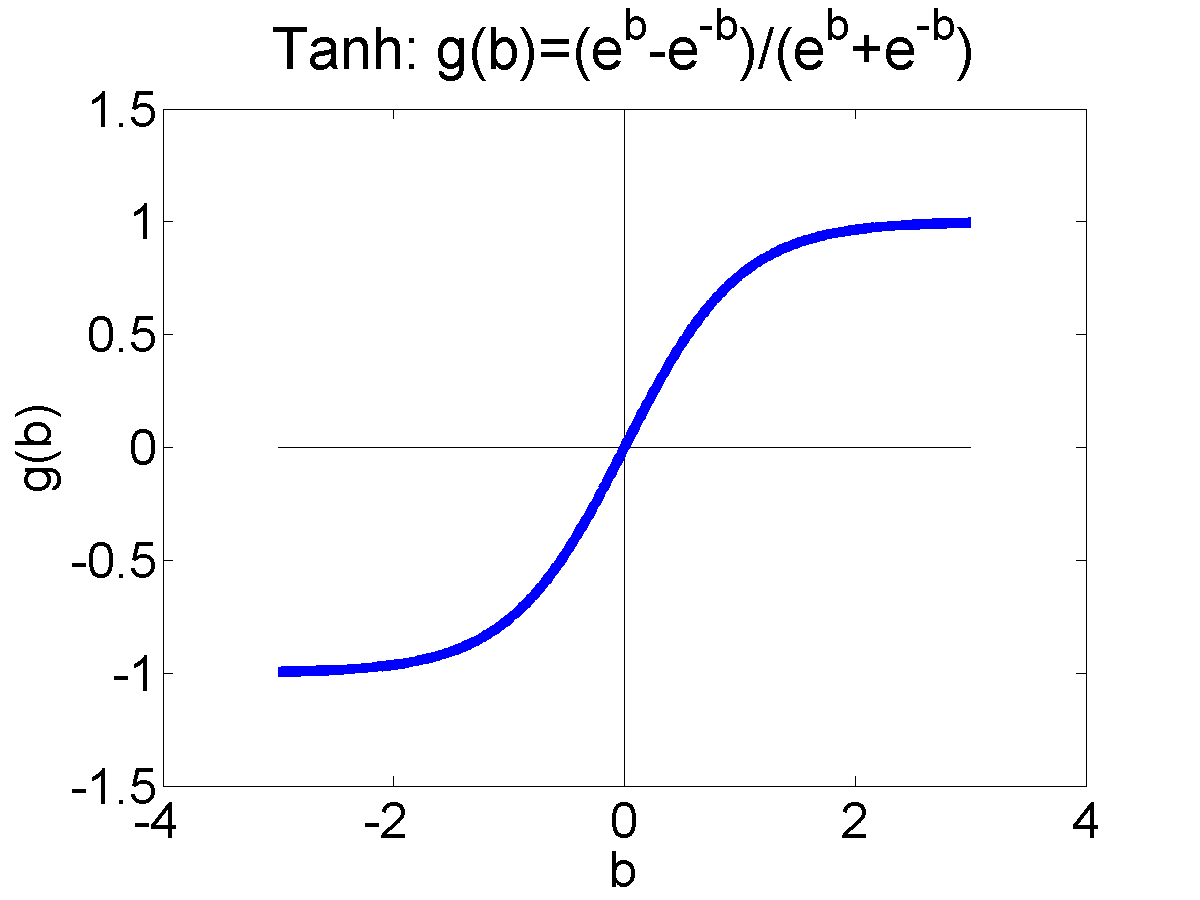
\includegraphics[width=1.75in]{figs/nn_tanh.png}}
    \end{block}
  \end{columns}
\end{frame}

\begin{frame}
  \frametitle{First Layer = A Series of Decisions}

  The first layer of the network decides whether or not to ``turn on'' each of the
  $h_j$'s.  It does this by comparing $\vec{x}$ to a series of linear threshold vectors:
  \[
  h_k = \sigma\left(\bar{w}_k^{(1)}\vec{x}\right)\approx\begin{cases}
  1 & \bar{w}_k^{(1)}\vec{x} > 0\\
  0 & \bar{w}_k^{(1)}\vec{x} < 0
  \end{cases}
  \]
\end{frame}

\begin{frame}
  \frametitle{Example \#2: Semicircle $\rightarrow$ Parabola}

  \centerline{\animategraphics[loop,controls,height=1.5in]{0.5}{exp/nnapprox}{0}{8}}
\end{frame}

%%%%%%%%%%%%%%%%%%%%%%%%%%%%%%%%%%%%%%%%%%%%%
\section[Learning]{Learning: Gradient Descent  and Back-Propagation}
\setcounter{subsection}{1}

\begin{frame}
  \frametitle{How to train a neural network}
  \begin{enumerate}
  \item Find a {\bf training dataset} that contains $n$ examples showing the
    desired output, $\vec{y}_i$, that the NN should compute in
    response to input vector $\vec{x}_i$:
    \[
    {\mathcal D}=\left\{(\vec{x}_1,\vec{y}_1),\ldots,(\vec{x}_n,\vec{y}_n)\right\}
    \]
    \item Randomly {\bf initialize} the weights and biases, $W^{(1)}$,
      $\vec{b}^{(1)}$, $W^{(2)}$, and $\vec{b}^{(2)}$.
    \item Perform {\bf forward propagation}: find out what the neural
      net computes as $\hat{y}_i$ for each $\vec{x}_i$.
    \item Define a {\bf loss function} that measures
      how badly $\hat{y}$ differs from $\vec{y}$.
    \item Perform {\bf back propagation} to improve  $W^{(1)}$,
      $\vec{b}^{(1)}$, $W^{(2)}$, and $\vec{b}^{(2)}$.
    \item Repeat steps 3-5 until convergence.
  \end{enumerate}
\end{frame}

\begin{frame}
  \frametitle{Loss Function: How should $h(\vec{x})$ be
    ``similar to'' $h^*(\vec{x})$?}
  \begin{block}{Minimum Mean Squared Error (MMSE)}
    \[
    W^*,b^*=\arg\min {\mathcal L} = \arg\min\frac{1}{2n}\sum_{i=1}^n
    \Vert\vec{y}_{i}-\hat{y}(\vec{x}_i)\Vert^2
    \]
  \end{block}
  \begin{block}{MMSE Solution: $\hat{y}\rightarrow E\left[\vec{y}|\vec{x}\right]$}
    If the training samples $(\vec{x}_i,\vec{y}_i)$ are i.i.d., then
    \[
    \lim_{n\rightarrow\infty}{\mathcal L} = \frac{1}{2}E\left[\Vert\vec{y}-\hat{y}\Vert^2\right]
    \]
    which is minimized by
    \[
    \hat{y}_{MMSE}(\vec{x})=E\left[\vec{y}|\vec{x}\right]
    \]
  \end{block}
\end{frame}

\begin{frame}
  \frametitle{Gradient Descent: How do we improve $W$ and $b$?}  Given
  some initial neural net parameter (called $u_{kj}$ in this figure),
  we want to find a better value of the same parameter.  We do that
  using gradient descent:
  \[
  u_{kj} \leftarrow u_{kj}-\eta\frac{d{\mathcal L}}{du_{kj}},
  \]
  where $\eta$ is a learning rate (some small constant, e.g., $\eta=0.02$ or so).
  \centerline{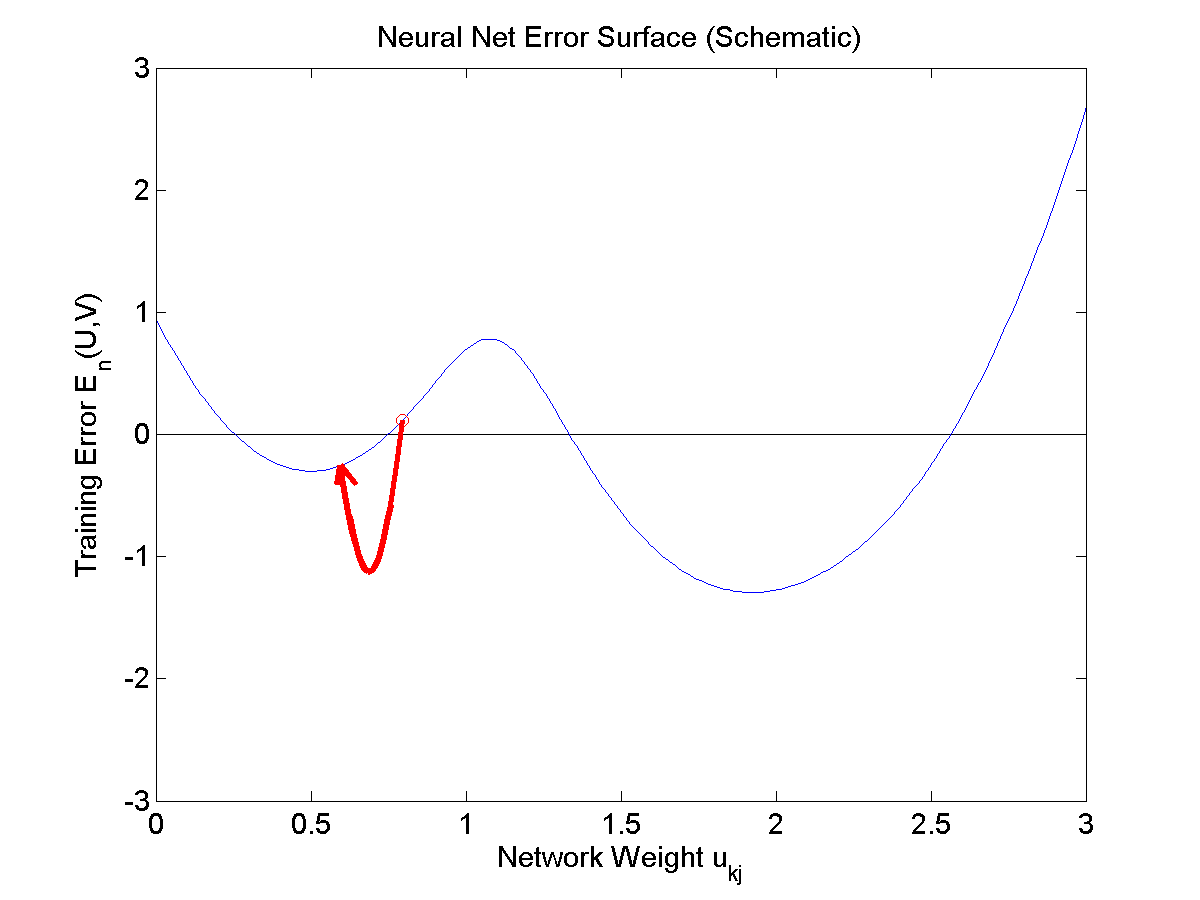
\includegraphics[width=2in]{figs/nn_errorsurf1.png}}
\end{frame}

\begin{frame}
\begin{block}{Gradient Descent = Local Optimization}
  Given an initial $W,b$, find new values of $W$, $b$ with lower error.
  \begin{align*}
    w_{kj}^{(1)} &\leftarrow w_{kj}^{(1)}-\eta\frac{d{\mathcal L}}{d w_{kj}^{(1)}}\\
    w_{kj}^{(2)} &\leftarrow w_{kj}^{(2)}-\eta\frac{d{\mathcal L}}{d w_{kj}^{(2)}}
  \end{align*}
\end{block}
\begin{block}{$\eta=$Learning Rate}
    \begin{itemize}
      \item If $\eta$ too large, gradient descent won't converge. If
        too small, convergence is slow.
      \item Second-order methods like L-BFGS and Adam choose an optimal $\eta$
        at each step, so they're MUCH faster.
    \end{itemize}
\end{block}
\end{frame}

\begin{frame}
  \frametitle{Computing the Gradient: Notation}
  \begin{itemize}
  \item $\vec{x}_i=[x_{1i},\ldots,x_{Di}]^T$ is the $i^{\textrm{th}}$ input vector.
  \item $\vec{y}_i=[y_{1i},\ldots,y_{Ki}]^T$ is the $i^{\textrm{th}}$ target vector (desired output).
  \item $\hat{y}_i=[\hat{y}_{1i},\ldots,\hat{y}_{Ki}]^T$ is the
    $i^{\textrm{th}}$ hypothesis vector (computed output).
  \item $\vec{e}_i^{(l)}=[e_{1i}^{(l)},\ldots,e_{Ni}^{(l)}]^T$ is the
    excitation vector after the $l^{\textrm{th}}$ layer, in response
    to the $i^{\textrm{th}}$ input.
  \item $\vec{h}_i=[h_{1i},\ldots,h_{Ni}]^T$ is the hidden nodes
    activation vector in response to the $i^{\textrm{th}}$ input. (No
     superscript necessary if there's only one hidden layer).
  \item The weight matrix for the $l^{\textrm{th}}$ layer is
    \[
    W^{(l)}=\left[\vec{w}_1^{(l)},\ldots,\vec{w}_j^{(l)},\ldots\right]=
    \left[\begin{array}{cccc}
        w_{11}^{(l)}&\cdots&w_{1j}^{(l)}&\cdots\\
        \vdots &\ddots&\vdots&\ddots\\
        w_{k1}^{(l)}&\cdots&w_{kj}^{(l)}&\cdots\\
        \vdots &\ddots&\vdots&\ddots
      \end{array}\right]
    \]
  \end{itemize}
\end{frame}
      
\begin{frame}
  \frametitle{Two-Layer Feedforward Neural Network}
  \begin{small}\begin{center}
  \tikzstyle{pre}=[<-,shorten <=1pt,>=stealth',semithick,draw=blue]
  \tikzstyle{post}=[->,shorten >=1pt,>=stealth',semithick,draw=blue]
  \begin{tikzpicture}[
      open/.style={circle,thick, draw=blue, text=black, align=left, text width=0.5cm}
    ]
    \node (x0) at (0,0.25) {$1$};
    \node[open] (x1) at (1,0) {$x_1$};
    \node[open] (x2) at (2,0) {$x_2$};
    \node (x3) at (2.75,0) {\ldots};
    \node[open] (xm0) at (3.5,0) {$x_{m_0}$};
    \node (input) at (6,0) {$\mathbf{a}_0=\mathbf{x}$ is the input vector};
    \node[open] (z11) at (1,1.3) {$z_{1,1}$} edge[pre](x0) edge[pre](x1) edge[pre](x2) edge[pre](xm0);
    \node[open] (z12) at (2,1.3) {$z_{1,2}$} edge[pre](x0) edge[pre](x1) edge[pre](x2) edge[pre](xm0);
    \node (z13) at (2.75,1.3) {\ldots};
    \node[open] (z1m1) at (3.5,1.3) {$z_{1,m_1}$} edge[pre](x0) edge[pre](x1) edge[pre](x2) edge[pre](xm0);
    \node (z1eq) at (6,1.3) {$\mathbf{z}_1=\mathbf{W}_1\mathbf{x}+\mathbf{b}_1$};
    \node (a10) at (0,2.7) {$1$};
    \node[open] (a11) at (1,2.45) {$a_{1,1}$} edge[pre](z11);
    \node[open] (a12) at (2,2.45) {$a_{1,2}$} edge[pre](z12);
    \node (a13) at (2.75,2.45) {\ldots};
    \node[open] (a1m1) at (3.5,2.45) {$a_{1,m_1}$} edge[pre](z1m1);
    \node (a1eq) at (6,2.45) {$\mathbf{a}_1=\mathbf{f}_1(\mathbf{z}_1)$};
    \node[open] (z21) at (1,3.75) {$z_{2,1}$} edge[pre](a10) edge[pre](a11) edge[pre](a12) edge[pre](a1m1);
    \node[open] (z22) at (2,3.75) {$z_{2,2}$} edge[pre](a10) edge[pre](a11) edge[pre](a12) edge[pre](a1m1);
    \node (z23) at (2.75,3.75) {\ldots};
    \node[open] (z2m2) at (3.5,3.75){$z_{2,m_2}$}edge[pre](a10) edge[pre](a11) edge[pre](a12) edge[pre](a1m1);
    \node (z2eq) at (6,3.75) {$\mathbf{z}_2=\mathbf{W}_2\mathbf{a}_1+\mathbf{b}_2$};
    \node[open] (a21) at (1,4.9) {$g_{1}$} edge[pre](z21);
    \node[open] (a22) at (2,4.9) {$g_{2}$} edge[pre](z22);
    \node (a23) at (2.75,4.9) {\ldots};
    \node[open] (a2m2) at (3.5,4.9) {$g_{m_2}$} edge[pre](z2m2);
    \node (z2eq) at (6,4.9) {$\mathbf{g}(\mathbf{x})=\mathbf{a}_2=\mathbf{f}_2(\mathbf{z}_2)$};
    \node (output) at (2.2,5.65) {${\mathcal{L}}=E\left[-\ln\Pr(\mathbf{y}|\mathbf{g}(\mathbf{x}))\right]$};
  \end{tikzpicture}
\end{center}
\end{small}
\end{frame}

\begin{frame}
  \frametitle{Computing the Derivative}
  OK, let's compute the derivative of ${\mathcal L}$ with respect to the $W^{(2)}$
  matrix.  Remember that $W^{(2)}$ enters the neural net computation as
  $e_{ki}^{(2)}=\sum_k w_{kj}^{(2)}h_{ji}$.  So\ldots
  \begin{align*}
    \frac{d{\mathcal L}}{dw_{kj}^{(2)}} &=
    \sum_{i=1}^n
    \left(\frac{\partial{\mathcal L}}{\partial e_{ki}^{(2)}}\right)
    \left(\frac{\partial e_{ki}^{(2)}}{\partial w_{kj}^{(2)}}\right)\\
    &= \sum_{i=1}^n \epsilon_{ki}h_{ki}
  \end{align*}
  where the last line only works if we define $\epsilon_{ki}$ in
  a useful way:
  \begin{align*}
    \vec\epsilon_i &= [\epsilon_{1i},\ldots,\epsilon_{Ki}]^T \\
    &= \nabla_{\vec{e}_{i}^{(2)}}{\mathcal L}~~~
    \left(\mbox{meaning that}~\epsilon_{ki}=\frac{\partial{\mathcal L}}{\partial e_{ki}^{(2)}}\right)\\
    &= \frac{1}{n}(\hat{y}_{i}-\vec{y}_{i})
  \end{align*}
\end{frame}

\begin{frame}
  \frametitle{Digression: Total Derivative vs.~Partial Derivative}
  \begin{itemize}
  \item The notation $\frac{d{\mathcal L}}{dw_{kj}^{(2)}}$ means
    ``the total derivative of ${\mathcal L}$ with respect to
    $w_{kj}^{(2)}$.'' It implies that we have to add up several
    different ways in which ${\mathcal L}$ depends on
    $w_{kj}^{(2)}$, for example,
    \begin{align*}
      \frac{d{\mathcal L}}{dw_{kj}^{(2)}} &=
      \sum_{i=1}^n
      \left(\frac{\partial{\mathcal L}}{\partial\hat{y}_{ki}}\right)
      \left(\frac{\partial\hat{y}_{ki}}{\partial w_{kj}^{(2)}}\right)
    \end{align*}
  \item The notation $\frac{\partial{\mathcal
      L}}{\partial\hat{y}_{ki}}$ means ``partial derivative.''  It
    means ``hold other variables constant while calculating this
    derivative.''
  \item For some variables, the total derivative and partial
    derivative are the same---it doesn't matter whether we hold other
    variables constant or not.  In fact, $\hat{y}_{ki}$ is one of
    those, so we could write $\frac{d{\mathcal
        L}}{d\hat{y}_{ki}}=\frac{\partial{\mathcal
        L}}{\partial\hat{y}_{ki}}$ for this particular variable.
  \item On the other hand, the difference starts to matter when we try
    to compute $\frac{d{\mathcal L}}{d w_{kj}^{(1)}}$.
  \end{itemize}
\end{frame}

\begin{frame}
  \begin{small}\begin{center}
  \tikzstyle{pre}=[<-,shorten <=1pt,>=stealth',semithick,draw=blue]
  \tikzstyle{post}=[->,shorten >=1pt,>=stealth',semithick,draw=blue]
  \begin{tikzpicture}[
      open/.style={circle,thick, draw=blue, text=black, align=left, text width=0.5cm}
    ]
    \node (x0) at (0,0.25) {$1$};
    \node[open] (x1) at (1,0) {$x_1$};
    \node[open] (x2) at (2,0) {$x_2$};
    \node (x3) at (2.75,0) {\ldots};
    \node[open] (xm0) at (3.5,0) {$x_{m_0}$};
    \node (input) at (6,0) {$\mathbf{a}_0=\mathbf{x}$ is the input vector};
    \node[open] (z11) at (1,1.3) {$z_{1,1}$} edge[pre](x0) edge[pre](x1) edge[pre](x2) edge[pre](xm0);
    \node[open] (z12) at (2,1.3) {$z_{1,2}$} edge[pre](x0) edge[pre](x1) edge[pre](x2) edge[pre](xm0);
    \node (z13) at (2.75,1.3) {\ldots};
    \node[open] (z1m1) at (3.5,1.3) {$z_{1,m_1}$} edge[pre](x0) edge[pre](x1) edge[pre](x2) edge[pre](xm0);
    \node (z1eq) at (6,1.3) {$\mathbf{z}_1=\mathbf{W}_1\mathbf{x}+\mathbf{b}_1$};
    \node (a10) at (0,2.7) {$1$};
    \node[open] (a11) at (1,2.45) {$a_{1,1}$} edge[pre](z11);
    \node[open] (a12) at (2,2.45) {$a_{1,2}$} edge[pre](z12);
    \node (a13) at (2.75,2.45) {\ldots};
    \node[open] (a1m1) at (3.5,2.45) {$a_{1,m_1}$} edge[pre](z1m1);
    \node (a1eq) at (6,2.45) {$\mathbf{a}_1=\mathbf{f}_1(\mathbf{z}_1)$};
    \node[open] (z21) at (1,3.75) {$z_{2,1}$} edge[pre](a10) edge[pre](a11) edge[pre](a12) edge[pre](a1m1);
    \node[open] (z22) at (2,3.75) {$z_{2,2}$} edge[pre](a10) edge[pre](a11) edge[pre](a12) edge[pre](a1m1);
    \node (z23) at (2.75,3.75) {\ldots};
    \node[open] (z2m2) at (3.5,3.75){$z_{2,m_2}$}edge[pre](a10) edge[pre](a11) edge[pre](a12) edge[pre](a1m1);
    \node (z2eq) at (6,3.75) {$\mathbf{z}_2=\mathbf{W}_2\mathbf{a}_1+\mathbf{b}_2$};
    \node[open] (a21) at (1,4.9) {$g_{1}$} edge[pre](z21);
    \node[open] (a22) at (2,4.9) {$g_{2}$} edge[pre](z22);
    \node (a23) at (2.75,4.9) {\ldots};
    \node[open] (a2m2) at (3.5,4.9) {$g_{m_2}$} edge[pre](z2m2);
    \node (z2eq) at (6,4.9) {$\mathbf{g}(\mathbf{x})=\mathbf{a}_2=\mathbf{f}_2(\mathbf{z}_2)$};
    \node (output) at (2.2,5.65) {${\mathcal{L}}=E\left[-\ln\Pr(\mathbf{y}|\mathbf{g}(\mathbf{x}))\right]$};
  \end{tikzpicture}
\end{center}
\end{small}
  \begin{block}{Back-Propagating to the First Layer}    
    \[
    \frac{d{\mathcal L}}{d w_{kj}^{(1)}} =
    \sum_{i=1}^n
    \left(\frac{d{\mathcal L}}{de_{ki}^{(1)}}\right)
    \left(\frac{\partial e_{ki}^{(1)}}{\partial w_{kj}^{(1)}}\right)
    = \sum_{i=1}^n \delta_{ki}x_{ji}
    \]
    \[
    \mbox{where:}~~\delta_{ki}=\frac{d{\mathcal L}}{de_{ki}^{(1)}}
    \]
  \end{block}
\end{frame}

\begin{frame}
  \begin{small}\begin{center}
  \tikzstyle{pre}=[<-,shorten <=1pt,>=stealth',semithick,draw=blue]
  \tikzstyle{post}=[->,shorten >=1pt,>=stealth',semithick,draw=blue]
  \begin{tikzpicture}[
      open/.style={circle,thick, draw=blue, text=black, align=left, text width=0.5cm}
    ]
    \node (x0) at (0,0.25) {$1$};
    \node[open] (x1) at (1,0) {$x_1$};
    \node[open] (x2) at (2,0) {$x_2$};
    \node (x3) at (2.75,0) {\ldots};
    \node[open] (xm0) at (3.5,0) {$x_{m_0}$};
    \node (input) at (6,0) {$\mathbf{a}_0=\mathbf{x}$ is the input vector};
    \node[open] (z11) at (1,1.3) {$z_{1,1}$} edge[pre](x0) edge[pre](x1) edge[pre](x2) edge[pre](xm0);
    \node[open] (z12) at (2,1.3) {$z_{1,2}$} edge[pre](x0) edge[pre](x1) edge[pre](x2) edge[pre](xm0);
    \node (z13) at (2.75,1.3) {\ldots};
    \node[open] (z1m1) at (3.5,1.3) {$z_{1,m_1}$} edge[pre](x0) edge[pre](x1) edge[pre](x2) edge[pre](xm0);
    \node (z1eq) at (6,1.3) {$\mathbf{z}_1=\mathbf{W}_1\mathbf{x}+\mathbf{b}_1$};
    \node (a10) at (0,2.7) {$1$};
    \node[open] (a11) at (1,2.45) {$a_{1,1}$} edge[pre](z11);
    \node[open] (a12) at (2,2.45) {$a_{1,2}$} edge[pre](z12);
    \node (a13) at (2.75,2.45) {\ldots};
    \node[open] (a1m1) at (3.5,2.45) {$a_{1,m_1}$} edge[pre](z1m1);
    \node (a1eq) at (6,2.45) {$\mathbf{a}_1=\mathbf{f}_1(\mathbf{z}_1)$};
    \node[open] (z21) at (1,3.75) {$z_{2,1}$} edge[pre](a10) edge[pre](a11) edge[pre](a12) edge[pre](a1m1);
    \node[open] (z22) at (2,3.75) {$z_{2,2}$} edge[pre](a10) edge[pre](a11) edge[pre](a12) edge[pre](a1m1);
    \node (z23) at (2.75,3.75) {\ldots};
    \node[open] (z2m2) at (3.5,3.75){$z_{2,m_2}$}edge[pre](a10) edge[pre](a11) edge[pre](a12) edge[pre](a1m1);
    \node (z2eq) at (6,3.75) {$\mathbf{z}_2=\mathbf{W}_2\mathbf{a}_1+\mathbf{b}_2$};
    \node[open] (a21) at (1,4.9) {$g_{1}$} edge[pre](z21);
    \node[open] (a22) at (2,4.9) {$g_{2}$} edge[pre](z22);
    \node (a23) at (2.75,4.9) {\ldots};
    \node[open] (a2m2) at (3.5,4.9) {$g_{m_2}$} edge[pre](z2m2);
    \node (z2eq) at (6,4.9) {$\mathbf{g}(\mathbf{x})=\mathbf{a}_2=\mathbf{f}_2(\mathbf{z}_2)$};
    \node (output) at (2.2,5.65) {${\mathcal{L}}=E\left[-\ln\Pr(\mathbf{y}|\mathbf{g}(\mathbf{x}))\right]$};
  \end{tikzpicture}
\end{center}
\end{small}
  \begin{block}{Back-Propagating to the First Layer}    
    \begin{align*}
      \delta_{ki} &=\frac{d{\mathcal L}}{de_{ki}^{(1)}}\\
      &= \sum_{\ell=1}^K
      \left(\frac{\partial{\mathcal L}}{\partial e_{\ell i}^{(2)}}\right)
      \left(\frac{\partial e_{\ell i}^{(2)}}{\partial h_{ki}}\right)
      \left(\frac{\partial h_{ki}}{\partial e_{ki}^{(1)}}\right)
    \end{align*}
  \end{block}
\end{frame}

\begin{frame}
  \begin{small}\begin{center}
  \tikzstyle{pre}=[<-,shorten <=1pt,>=stealth',semithick,draw=blue]
  \tikzstyle{post}=[->,shorten >=1pt,>=stealth',semithick,draw=blue]
  \begin{tikzpicture}[
      open/.style={circle,thick, draw=blue, text=black, align=left, text width=0.5cm}
    ]
    \node (x0) at (0,0.25) {$1$};
    \node[open] (x1) at (1,0) {$x_1$};
    \node[open] (x2) at (2,0) {$x_2$};
    \node (x3) at (2.75,0) {\ldots};
    \node[open] (xm0) at (3.5,0) {$x_{m_0}$};
    \node (input) at (6,0) {$\mathbf{a}_0=\mathbf{x}$ is the input vector};
    \node[open] (z11) at (1,1.3) {$z_{1,1}$} edge[pre](x0) edge[pre](x1) edge[pre](x2) edge[pre](xm0);
    \node[open] (z12) at (2,1.3) {$z_{1,2}$} edge[pre](x0) edge[pre](x1) edge[pre](x2) edge[pre](xm0);
    \node (z13) at (2.75,1.3) {\ldots};
    \node[open] (z1m1) at (3.5,1.3) {$z_{1,m_1}$} edge[pre](x0) edge[pre](x1) edge[pre](x2) edge[pre](xm0);
    \node (z1eq) at (6,1.3) {$\mathbf{z}_1=\mathbf{W}_1\mathbf{x}+\mathbf{b}_1$};
    \node (a10) at (0,2.7) {$1$};
    \node[open] (a11) at (1,2.45) {$a_{1,1}$} edge[pre](z11);
    \node[open] (a12) at (2,2.45) {$a_{1,2}$} edge[pre](z12);
    \node (a13) at (2.75,2.45) {\ldots};
    \node[open] (a1m1) at (3.5,2.45) {$a_{1,m_1}$} edge[pre](z1m1);
    \node (a1eq) at (6,2.45) {$\mathbf{a}_1=\mathbf{f}_1(\mathbf{z}_1)$};
    \node[open] (z21) at (1,3.75) {$z_{2,1}$} edge[pre](a10) edge[pre](a11) edge[pre](a12) edge[pre](a1m1);
    \node[open] (z22) at (2,3.75) {$z_{2,2}$} edge[pre](a10) edge[pre](a11) edge[pre](a12) edge[pre](a1m1);
    \node (z23) at (2.75,3.75) {\ldots};
    \node[open] (z2m2) at (3.5,3.75){$z_{2,m_2}$}edge[pre](a10) edge[pre](a11) edge[pre](a12) edge[pre](a1m1);
    \node (z2eq) at (6,3.75) {$\mathbf{z}_2=\mathbf{W}_2\mathbf{a}_1+\mathbf{b}_2$};
    \node[open] (a21) at (1,4.9) {$g_{1}$} edge[pre](z21);
    \node[open] (a22) at (2,4.9) {$g_{2}$} edge[pre](z22);
    \node (a23) at (2.75,4.9) {\ldots};
    \node[open] (a2m2) at (3.5,4.9) {$g_{m_2}$} edge[pre](z2m2);
    \node (z2eq) at (6,4.9) {$\mathbf{g}(\mathbf{x})=\mathbf{a}_2=\mathbf{f}_2(\mathbf{z}_2)$};
    \node (output) at (2.2,5.65) {${\mathcal{L}}=E\left[-\ln\Pr(\mathbf{y}|\mathbf{g}(\mathbf{x}))\right]$};
  \end{tikzpicture}
\end{center}
\end{small}
  \begin{block}{Back-Propagating to the First Layer}    
    \begin{align*}
      \delta_{ki} 
      &= \sum_{\ell=1}^K
      \left(\frac{\partial{\mathcal L}}{\partial e_{\ell i}^{(2)}}\right)
      \left(\frac{\partial e_{\ell i}^{(2)}}{\partial h_{ki}}\right)
      \left(\frac{\partial h_{ki}}{\partial e_{ki}^{(1)}}\right)\\
      &= \sum_{\ell=1}^K \epsilon_{\ell i}w_{\ell k}^{(2)}\sigma'(e_{ki}^{(1)})
    \end{align*}
  \end{block}
\end{frame}

\begin{frame}
  \begin{small}\begin{center}
  \tikzstyle{pre}=[<-,shorten <=1pt,>=stealth',semithick,draw=blue]
  \tikzstyle{post}=[->,shorten >=1pt,>=stealth',semithick,draw=blue]
  \begin{tikzpicture}[
      open/.style={circle,thick, draw=blue, text=black, align=left, text width=0.5cm}
    ]
    \node (x0) at (0,0.25) {$1$};
    \node[open] (x1) at (1,0) {$x_1$};
    \node[open] (x2) at (2,0) {$x_2$};
    \node (x3) at (2.75,0) {\ldots};
    \node[open] (xm0) at (3.5,0) {$x_{m_0}$};
    \node (input) at (6,0) {$\mathbf{a}_0=\mathbf{x}$ is the input vector};
    \node[open] (z11) at (1,1.3) {$z_{1,1}$} edge[pre](x0) edge[pre](x1) edge[pre](x2) edge[pre](xm0);
    \node[open] (z12) at (2,1.3) {$z_{1,2}$} edge[pre](x0) edge[pre](x1) edge[pre](x2) edge[pre](xm0);
    \node (z13) at (2.75,1.3) {\ldots};
    \node[open] (z1m1) at (3.5,1.3) {$z_{1,m_1}$} edge[pre](x0) edge[pre](x1) edge[pre](x2) edge[pre](xm0);
    \node (z1eq) at (6,1.3) {$\mathbf{z}_1=\mathbf{W}_1\mathbf{x}+\mathbf{b}_1$};
    \node (a10) at (0,2.7) {$1$};
    \node[open] (a11) at (1,2.45) {$a_{1,1}$} edge[pre](z11);
    \node[open] (a12) at (2,2.45) {$a_{1,2}$} edge[pre](z12);
    \node (a13) at (2.75,2.45) {\ldots};
    \node[open] (a1m1) at (3.5,2.45) {$a_{1,m_1}$} edge[pre](z1m1);
    \node (a1eq) at (6,2.45) {$\mathbf{a}_1=\mathbf{f}_1(\mathbf{z}_1)$};
    \node[open] (z21) at (1,3.75) {$z_{2,1}$} edge[pre](a10) edge[pre](a11) edge[pre](a12) edge[pre](a1m1);
    \node[open] (z22) at (2,3.75) {$z_{2,2}$} edge[pre](a10) edge[pre](a11) edge[pre](a12) edge[pre](a1m1);
    \node (z23) at (2.75,3.75) {\ldots};
    \node[open] (z2m2) at (3.5,3.75){$z_{2,m_2}$}edge[pre](a10) edge[pre](a11) edge[pre](a12) edge[pre](a1m1);
    \node (z2eq) at (6,3.75) {$\mathbf{z}_2=\mathbf{W}_2\mathbf{a}_1+\mathbf{b}_2$};
    \node[open] (a21) at (1,4.9) {$g_{1}$} edge[pre](z21);
    \node[open] (a22) at (2,4.9) {$g_{2}$} edge[pre](z22);
    \node (a23) at (2.75,4.9) {\ldots};
    \node[open] (a2m2) at (3.5,4.9) {$g_{m_2}$} edge[pre](z2m2);
    \node (z2eq) at (6,4.9) {$\mathbf{g}(\mathbf{x})=\mathbf{a}_2=\mathbf{f}_2(\mathbf{z}_2)$};
    \node (output) at (2.2,5.65) {${\mathcal{L}}=E\left[-\ln\Pr(\mathbf{y}|\mathbf{g}(\mathbf{x}))\right]$};
  \end{tikzpicture}
\end{center}
\end{small}
  \begin{block}{Back-Propagating to the First Layer}    
    \[
    \frac{d{\mathcal L}}{d w_{kj}^{(1)}} =
    \sum_{i=1}^n
    \left(\frac{d{\mathcal L}}{de_{ki}^{(1)}}\right)
    \left(\frac{\partial e_{ki}^{(1)}}{\partial w_{kj}^{(1)}}\right)
    = \sum_{i=1}^n \delta_{ki}x_{ji}
    \]
    \[
    \delta_{ki}=\frac{d{\mathcal L}}{de_{ki}^{(1)}}=
    \sum_{\ell=1}^K \epsilon_{\ell i}w_{\ell k}^{(2)}\sigma'(e_{ki}^{(1)})
    \]
  \end{block}
\end{frame}

\begin{frame}
  \begin{block}{The Back-Propagation Algorithm}
    \[
    W^{(2)}\leftarrow W^{(2)}-\eta\nabla_{W^{(2)}}{\mathcal L},~~~~~
    W^{(1)}\leftarrow W^{(1)}-\eta\nabla_{W^{(1)}}{\mathcal L}
    \]
    \[
    \nabla_{W^{(2)}}{\mathcal L}=\sum_{i=1}^n \vec\epsilon_i\vec{h}_i^T,~~~~~
    \nabla_{W^{(1)}}{\mathcal L}=\sum_{i=1}^n\vec\delta_i\vec{x}_i^T
    \]
    \[
    \epsilon_{ki}=\frac{1}{n} (\hat{y}_{ki}-y_{ki}),~~~~~
    \delta_{ki}=\sum_{\ell=1}^K \epsilon_{\ell i}w_{\ell k}^{(2)}\sigma'(e_{ki}^{(1)})
    \]
    \[
    \vec\epsilon_i=\frac{1}{n}\left(\hat{y}_i-\vec{y}_i\right),~~~~~
    \vec\delta_i=\sigma'(\vec{e}_i^{(1)})\odot W^{(2),T}\vec\epsilon_i
    \]
    \ldots where $\odot$ means element-wise multiplication of two
    vectors; $\sigma'(\vec{e})$ is the element-wise
    derivative of $\sigma(\vec{e})$.
  \end{block}
\end{frame}

\begin{frame}
  \frametitle{Derivatives of the Nonlinearities}
  \begin{columns}[t]
    \column{2.25in}
    \begin{block}{Logistic}
      \centerline{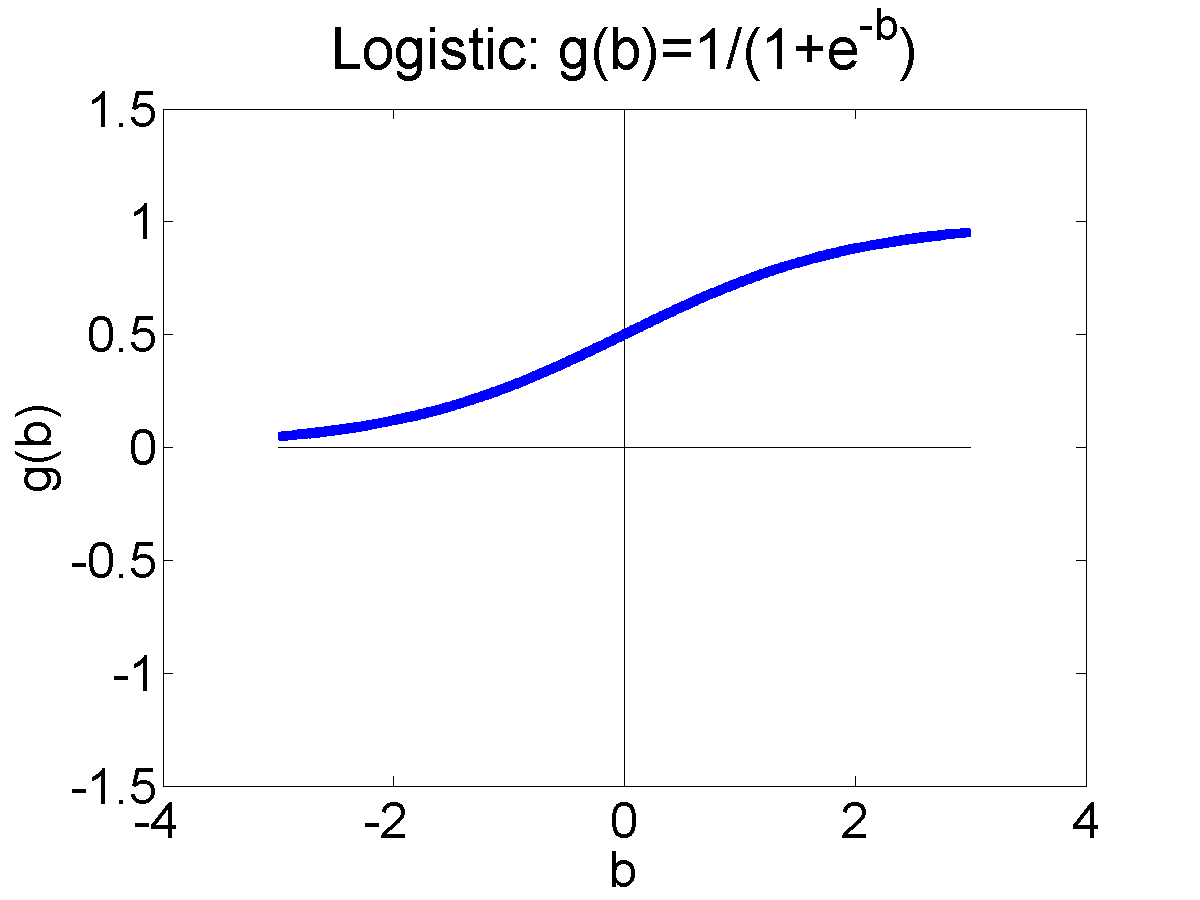
\includegraphics[width=1.75in]{figs/nn_logistic.png}}
      \centerline{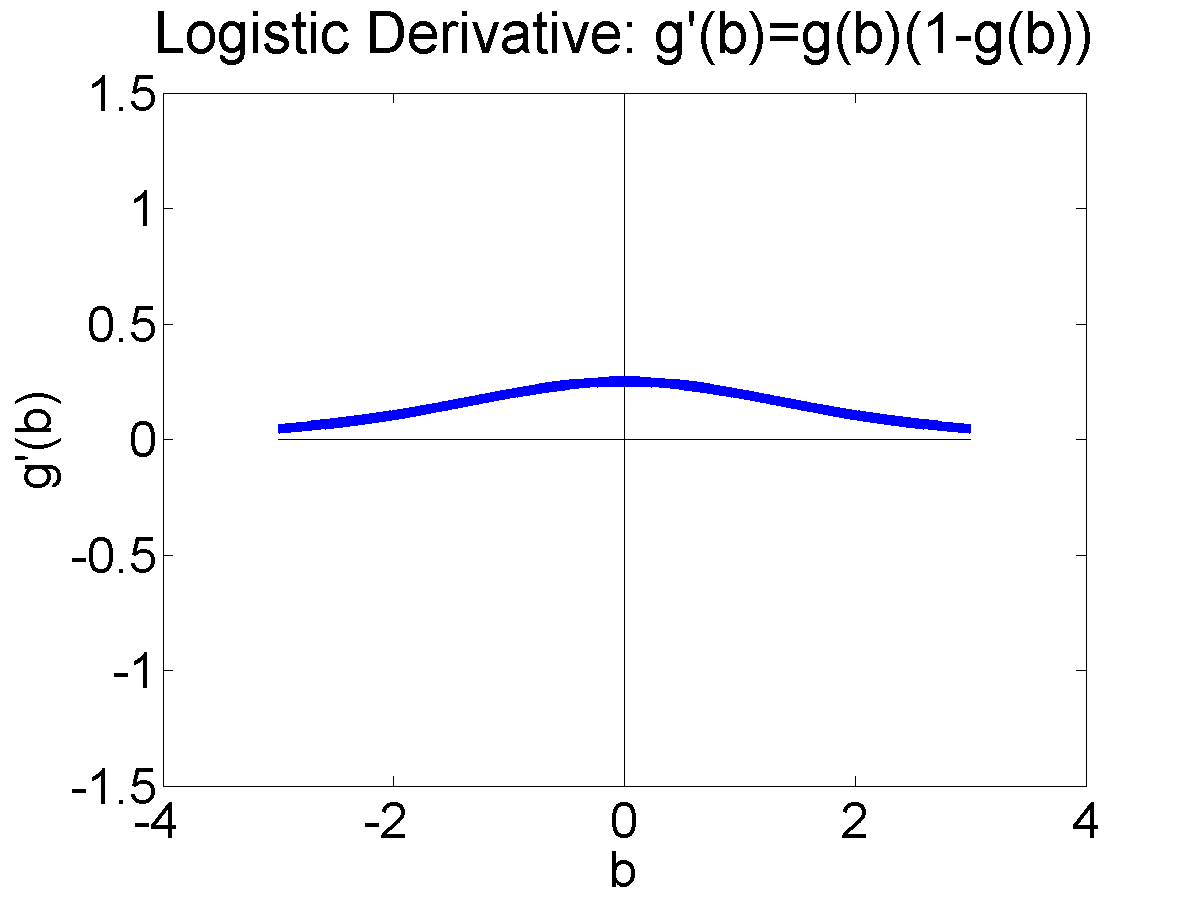
\includegraphics[width=1.75in]{figs/nn_logisticprime.png}}
    \end{block}
    \column{2.25in}
    \begin{block}{Tanh}
      \centerline{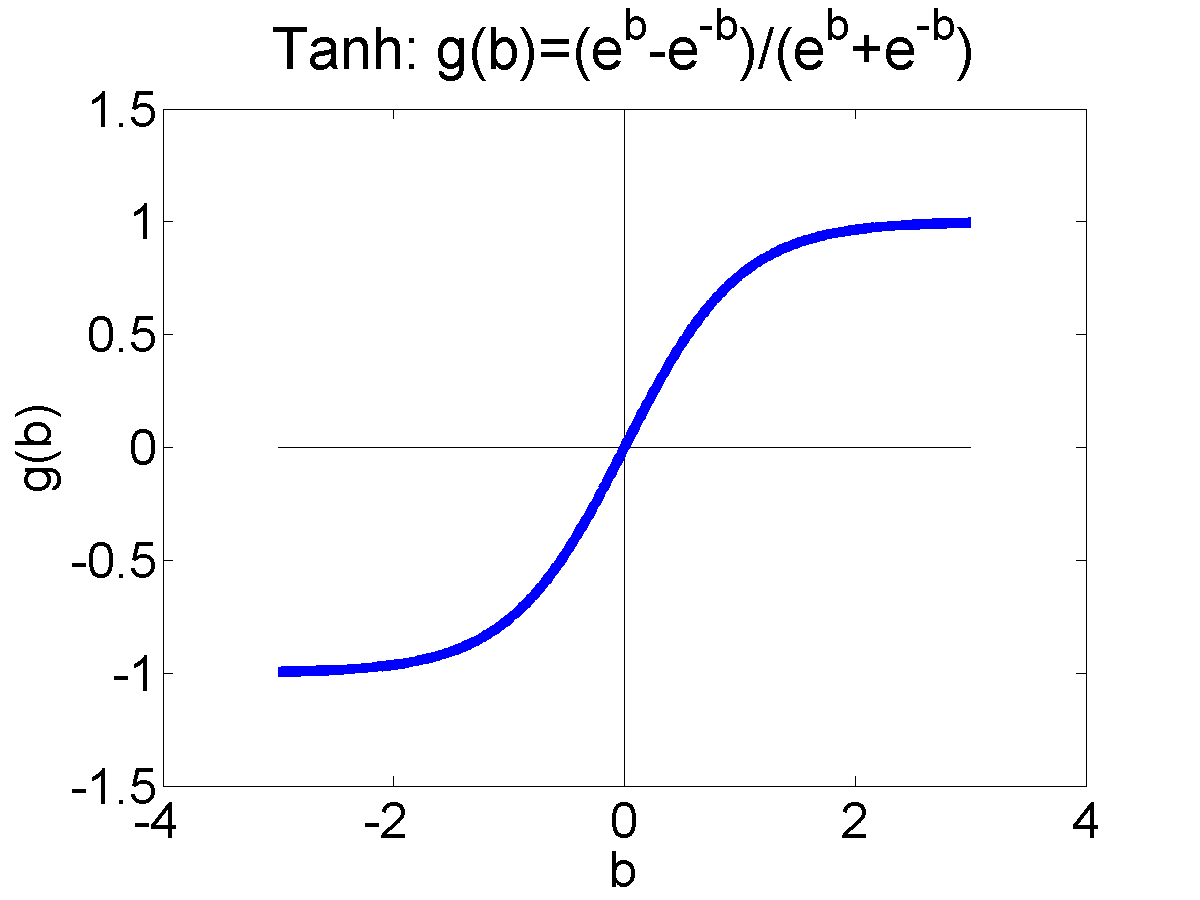
\includegraphics[width=1.75in]{figs/nn_tanh.png}}
      \centerline{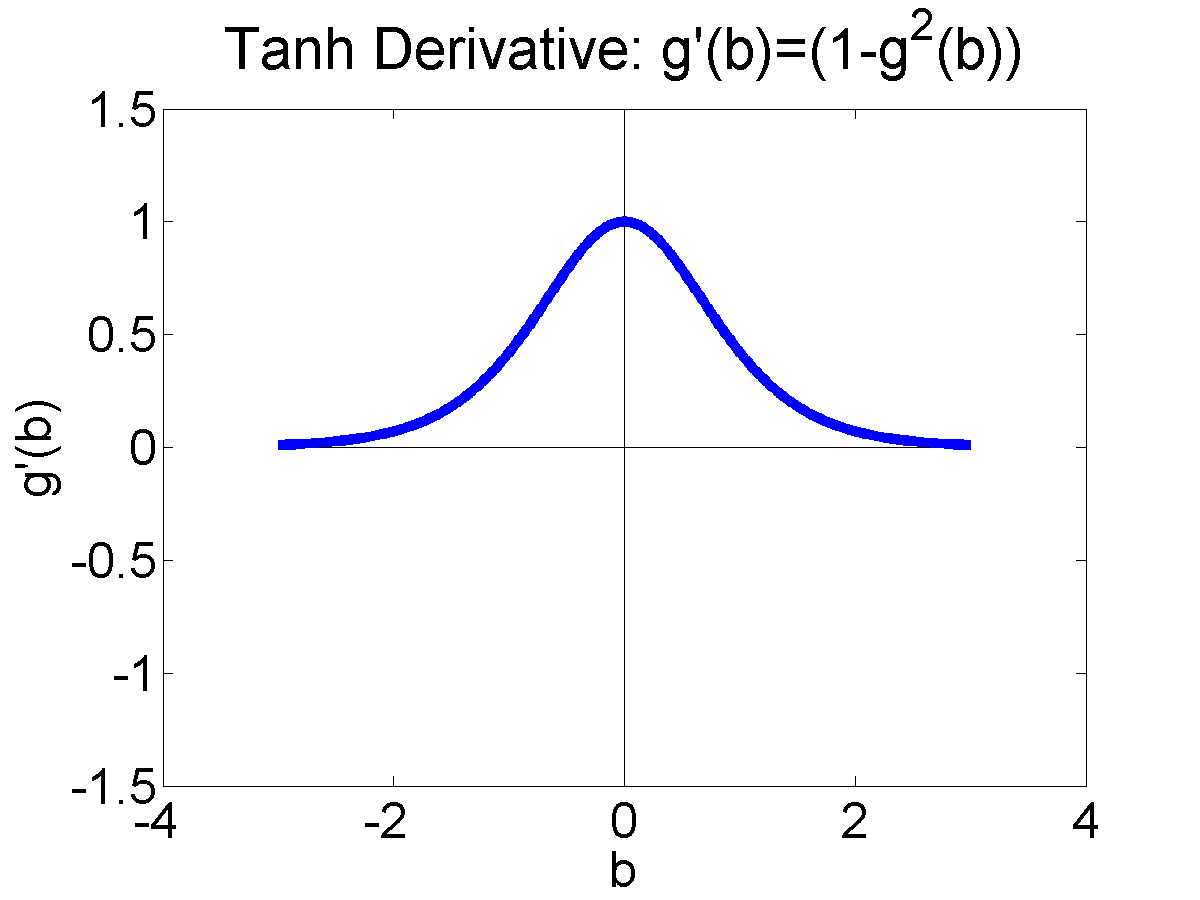
\includegraphics[width=1.75in]{figs/nn_tanhprime.png}}
    \end{block}
  \end{columns}
\end{frame}

%%%%%%%%%%%%%%%%%%%%%%%%%%%%%%%%%%%%%%%%%%%%%%%%%%%%%%%%%%%%%%%
\section[Backprop Example]{Backprop Example: Semicircle $\rightarrow$ Parabola}
\setcounter{subsection}{1}

\begin{frame}
  \frametitle{Backprop Example: Semicircle $\rightarrow$ Parabola}

  \centerline{\includegraphics[height=1.5in]{exp/nn_target_figure.png}}

  Remember, we are going to try to approximate this using:
  \[
  \hat{y} = \vec{b} + \sum_j \vec{w}_{j}^{(2)} \sigma\left(\bar{w}_{k}^{(1)} \vec{x}\right)
  \]
\end{frame}

\begin{frame}
  \frametitle{Randomly Initialized Weights}

  Here's what we get if we randomly initialize $\bar{w}_k^{(1)}$,
  $\vec{b}$, and $\vec{w}_j^{(2)}$.  The red vector on the right is
  the estimation error for this training token,
  $\vec\epsilon=\hat{y}-\vec{y}$.  It's huge!
  \centerline{\includegraphics[height=1.5in]{exp/nntrain_init.png}}
\end{frame}

\begin{frame}
  \frametitle{Back-Prop: Layer 2}
  Remember
  \begin{align*}
    W^{(2)} &\leftarrow W^{(2)}-\eta\nabla_{W^{(2)}}{\mathcal L}
    = W^{(2)}-\eta\sum_{i=1}^n \vec\epsilon_i\vec{h}_i^T\\
    &= W^{(2)}-\frac{\eta}{n}\sum_{i=1}^n \left(\hat{y}_i-\vec{y}_i\right)\vec{h}_i^T
  \end{align*}
  Thinking in terms of the columns of $W^{(2)}$, we have
  \[
  \vec{w}_j^{(2)} \leftarrow
  \vec{w}_j^{(2)}-\frac{\eta}{n}\sum_{i=1}^n \left(\hat{y}_i-\vec{y}_i\right)h_{ji}
  \]
  So, in words, layer-2 backprop means
  \begin{itemize}
  \item Each column, $\vec{w}_j^{(2)}$, gets updated in the direction
    $\vec{y}-\hat{y}$.
  \item The update for the $j^{\textrm{th}}$ column, in response to
    the $i^{\textrm{th}}$ training token, is scaled by its
    activation $h_{ji}$.
  \end{itemize}
\end{frame}

\begin{frame}
  \frametitle{Back-Prop: Layer 1}
  Remember
  \begin{align*}
    W^{(1)} &\leftarrow W^{(1)}-\eta\nabla_{W^{(1)}}{\mathcal L}
    = W^{(1)}-\eta\sum_{i=1}^n \vec\delta_i\vec{x}_i^T\\
    &= W^{(1)}-\eta\sum_{i=1}^n \left(\sigma'(\vec{e}_i^{(1)})\odot W^{(2),T}\vec\epsilon_i\right)\vec{x}_i^T
  \end{align*}
  Thinking in terms of the rows of $W^{(1)}$, we have
  \[
  \bar{w}_k^{(1)} \leftarrow
  \bar{w}_k^{(1)}-\eta\sum_{i=1}^n\delta_{ki}\vec{x}_i^T
  \]
  In words, layer-1 backprop means
  \begin{itemize}
  \item Each row, $\bar{w}_k^{(1)}$, gets updated in the direction
    $-\vec{x}$.
  \item The update for the $k^{\textrm{th}}$ row, in response to
    the $i^{\textrm{th}}$ training token, is scaled by its
    back-propagated error term $\delta_{ki}$.
  \end{itemize}
\end{frame}

\begin{frame}
  \frametitle{Back-Prop Example: Semicircle $\rightarrow$ Parabola}
  For each column $\vec{w}_j^{(2)}$ and the corresponding row $\bar{w}_k^{(1)}$,
  \[
  \vec{w}_j^{(2)} \leftarrow
  \vec{w}_j^{(2)}-\frac{\eta}{n}\sum_{i=1}^n \left(\hat{y}_i-\vec{y}_i\right)h_{ji},~~~~
  \bar{w}_k^{(1)} \leftarrow
  \bar{w}_k^{(1)}-\eta\sum_{i=1}^n\delta_{ki}\vec{x}_i^T
  \]
  \centerline{\animategraphics[loop,controls,height=1.5in]{20}{exp/nntrain}{0}{499}}
\end{frame}

%%%%%%%%%%%%%%%%%%%%%%%%%%%%%%%%%%%%%%%%%%%%
\section[Summary]{Summary}
\setcounter{subsection}{1}

\begin{frame}
  \frametitle{Summary}
  \begin{itemize}
  \item A neural network approximates an arbitrary function using a sort of piece-wise approximation.
  \item The activation of each piece is determined by a nonlinear activation function applied to
    the hidden layer.
  \item Training is done using gradient descent.
  \item ``Back-propagation'' is the process of using the chain rule of differentiation
    in order to find the derivative of the loss with respect to each of the learnable weights
    and biases of the network.
  \end{itemize}
\end{frame}
    
\end{document}

